\newpage
\section{Dùng công cụ Excel, SPSS, Python và R tính toán}

\subsection{Sử dụng Excel}
Sau khi mở file \texttt{VNZ\_STOCK\_DATA\_AUGUST.csv} trong Excel, 
tiến hành chuyển đổi và lưu lại dưới dạng file 
\texttt{VNZ\_STOCK\_DATA\_AUGUST.xlsx}.  

Tiếp theo, tạo một sheet mới với tên \texttt{Descriptive Stats} để thực hiện 
các thống kê mô tả dữ liệu.
\subsection*{Tính các chỉ số Central Tendency}

Trong sheet ``\texttt{Descriptive Statistics}'', tạo bảng như sau:

\begin{center}
\begin{tabular}{|l|l|}
\hline
\textbf{Chỉ số} & \textbf{Hàm Excel} \\
\hline
Mean              & \texttt{=AVERAGE(TotalValue)}          \\ \hline
Median            & \texttt{=MEDIAN(TotalValue)}           \\ \hline
Mode              & \texttt{=MODE.SNGL(TotalValue)}        \\ \hline
Q1 (Quartile 1)   & \texttt{=QUARTILE.INC(TotalValue,1)}   \\ \hline
Q2 (Quartile 2)   & \texttt{=QUARTILE.INC(TotalValue,2)}   \\ \hline
Q3 (Quartile 3)   & \texttt{=QUARTILE.INC(TotalValue,3)}   \\ \hline
\end{tabular}
\end{center}

\subsection*{Tính các chỉ số Dispersion}

\begin{center}
\begin{tabular}{|l|l|l|}
\hline
\textbf{Chỉ số} & \textbf{Công thức Excel}\\
\hline
Variance (Sample)         & \texttt{=VAR.S(TotalValue)}                                               \\ \hline
Standard Deviation        & \texttt{=STDEV.S(TotalValue)}                                            \\ \hline
Range                     & \texttt{=MAX(TotalValue)-MIN(TotalValue)}                             \\ \hline
Standard Error of Mean    & \texttt{=STDEV.S(TotalValue)/SQRT(COUNT(TotalValue))}                \\ \hline
Skewness                  & \texttt{=SKEW(TotalValue)}                                                \\ \hline
Kurtosis                  & \texttt{=KURT(TotalValue)}                                                \\ \hline
\end{tabular}
\end{center}

\newpage
\subsection*{Kết quả thu được}

\begin{figure}[!htp]
    \centering
    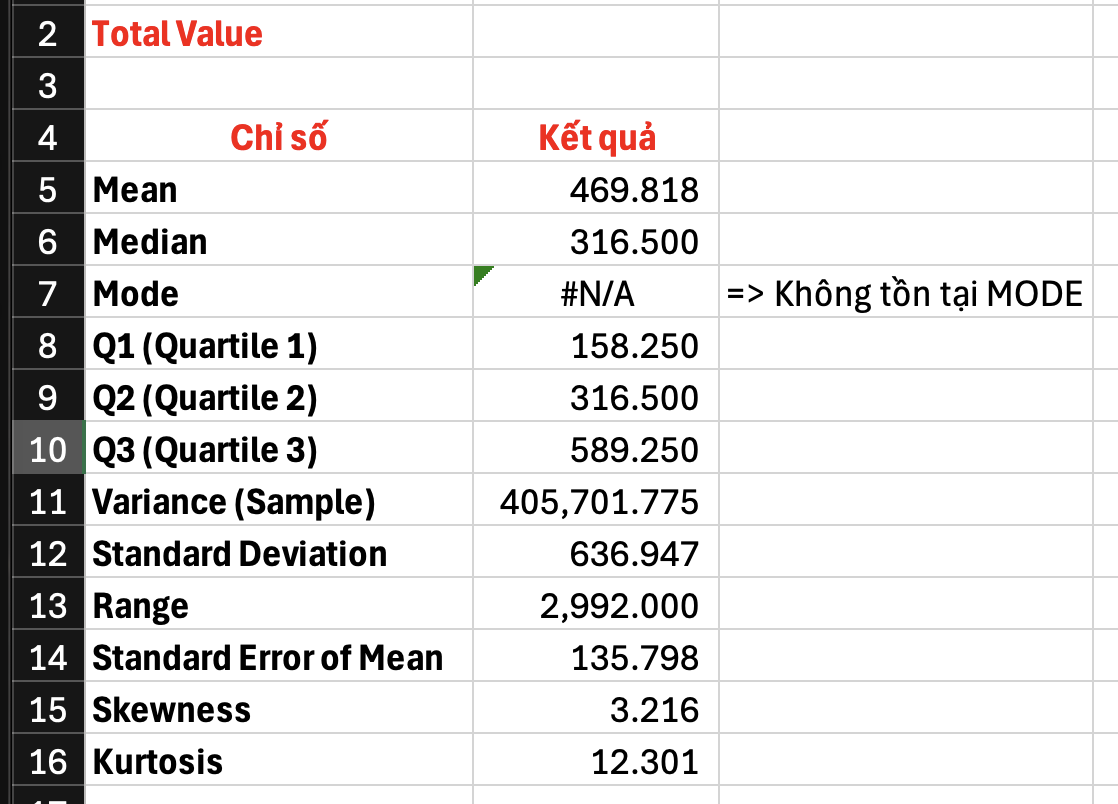
\includegraphics[width=0.6\textwidth]{LAB01/pics/Excel_Table.png}%
    \caption{Kết quả tính Descriptive Statistics từ Excel}
    \label{fig:Excel_Stats}
\end{figure}

\begin{figure}[!htp]
    \centering
    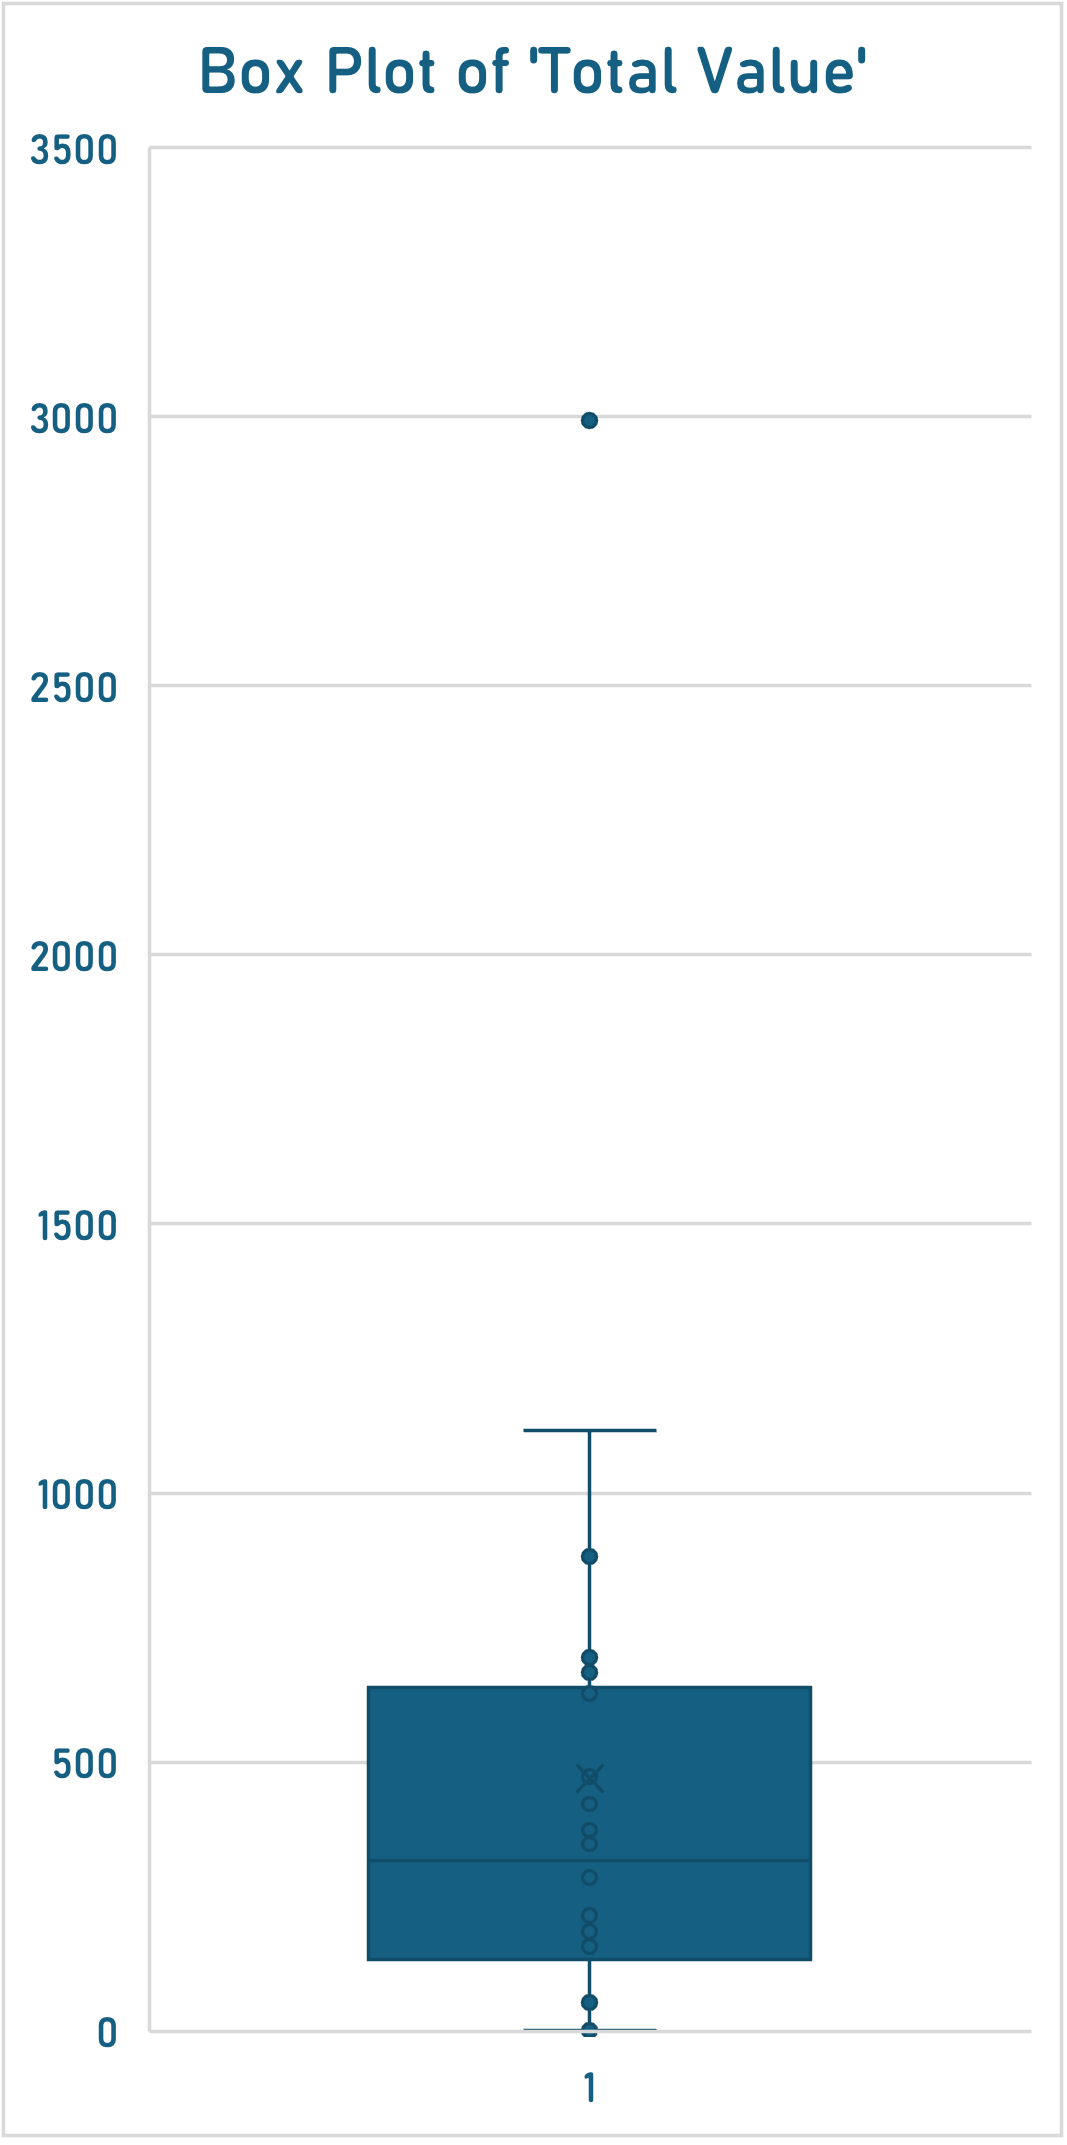
\includegraphics[width=0.4\textwidth]{LAB01/pics/Excel_BoxPlot.png}%
    \caption{Vẽ BoxPlot của cột \texttt{Total Value} từ Excel}
    \label{fig:Excel_BoxPlot}
\end{figure}

\begin{figure}[!htp]
    \centering
    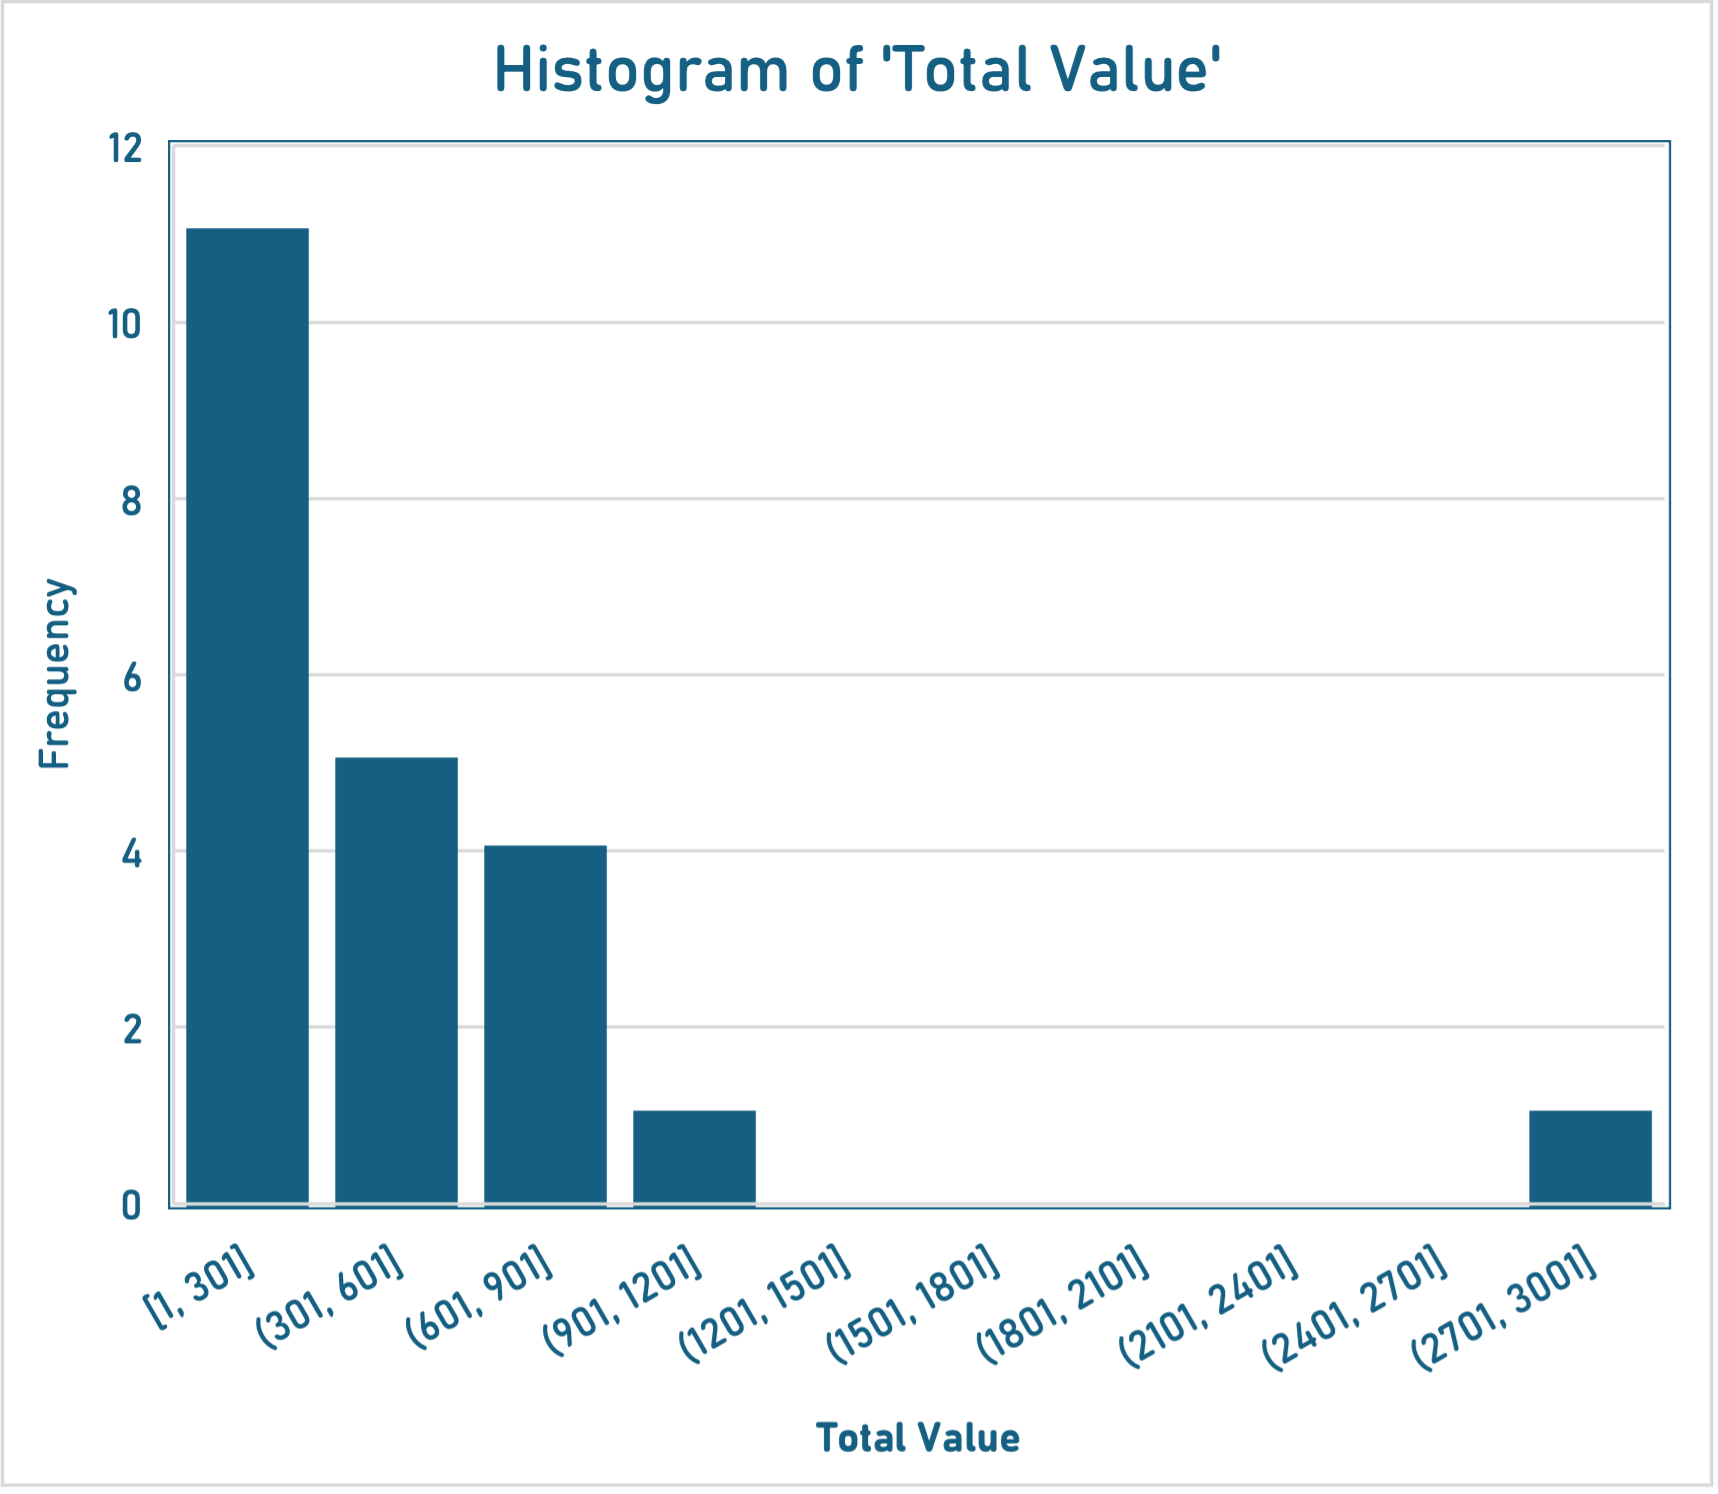
\includegraphics[width=0.8\textwidth]{LAB01/pics/Excel_Hist.png}%
    \caption{Vẽ Histogram của cột \texttt{Total Value} từ Excel}
    \label{fig:Excel_Hist}
\end{figure}


\subsection{SPSS}

Sử dụng phần mềm \textbf{IBM SPSS Statistics} để thực hiện phân tích thống kê mô tả (\textit{Descriptive Statistics}) cho bộ dữ liệu chứng khoán \texttt{VNZ\_STOCK\_DATA\_AUGUST.csv}.

Quy trình thống kê mô tả trong SPSS được thực hiện theo các bước sau:

\begin{enumerate}
    \item Mở phần mềm \textbf{SPSS Statistics}.
    
    \item Chọn menu:
    \[
    \texttt{File} \rightarrow \texttt{Open} \rightarrow \texttt{Data}
    \]
    và tải lên file dữ liệu \texttt{VNZ\_STOCK\_DATA\_AUGUST.csv}.
    
    \item Sau khi dữ liệu được import thành công, chọn tiếp:
    \[
    \texttt{Analyze} \rightarrow \texttt{Descriptive Statistics} \rightarrow \texttt{Frequency}
    \]
    
    \item Trong hộp thoại \texttt{Frequency}, để biến \texttt{TotalValue} vào mục \texttt{Dependent List}.
    
    \item Trong hộp thoại \texttt{Frequency: Statistics}, chọn như Hình \ref{fig:SPSS_Options}
    \begin{figure}[!htp]
    \centering
    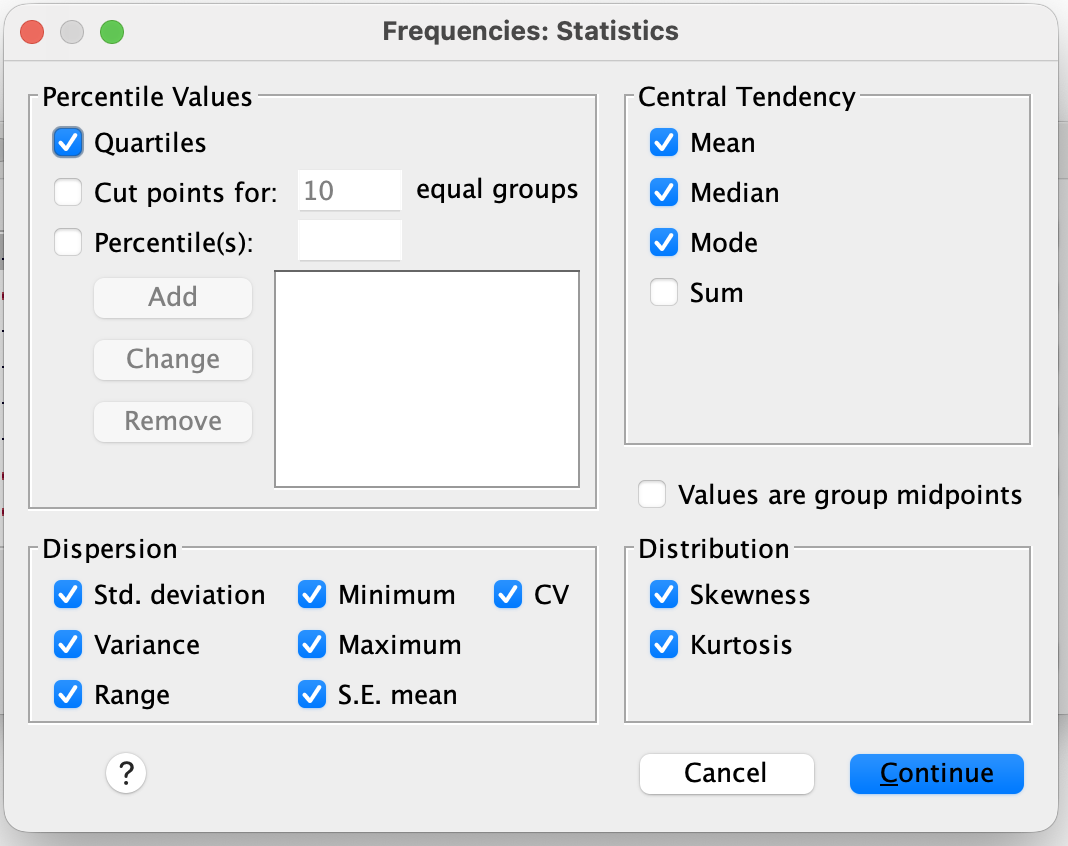
\includegraphics[width=.75\textwidth]{LAB01/pics/SPSS_Option_Frequency.png}%
    \caption{Các options cần chọn trong SPSS}
    \label{fig:SPSS_Options}
    \end{figure}   
    
    \item Cuối cùng, nhấn \texttt{OK} để SPSS xuất kết quả thống kê mô tả.
\end{enumerate}

\subsubsection*{Hình ảnh thu được}

\begin{figure}[!htp]
    \centering
    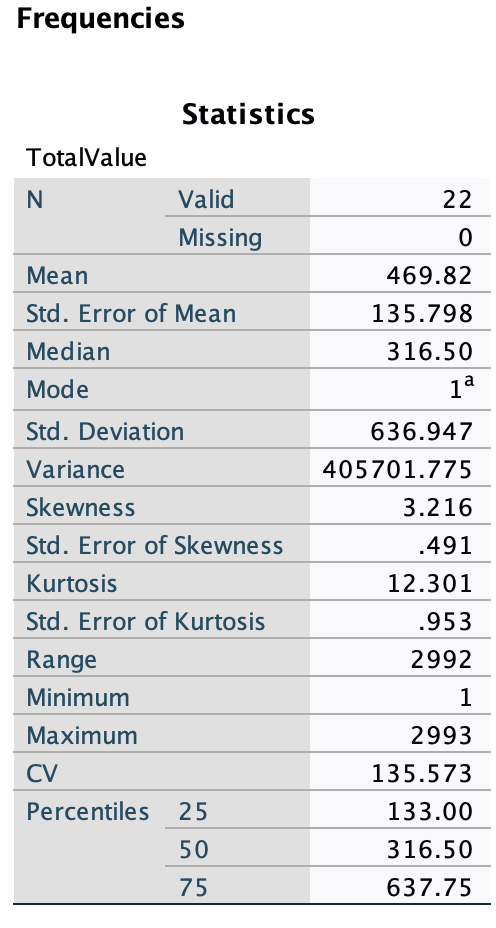
\includegraphics[width=0.7\textwidth]{LAB01/pics/SPSS_Table.png}%
    \caption{Kết quả tính Descriptive Statistics từ SPSS}
    \label{fig:SPSS_Stats}
\end{figure}


\begin{figure}[!htp]
    \centering
    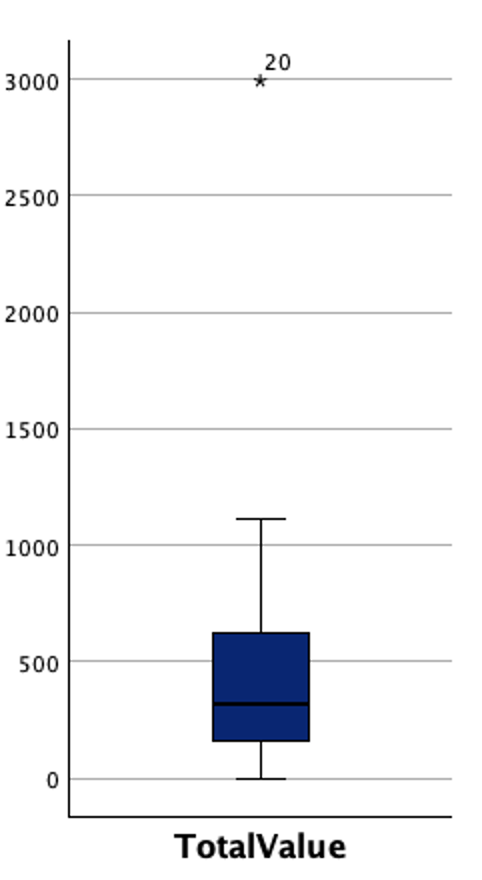
\includegraphics[width=0.4\textwidth]{LAB01/pics/SPSS_BoxPlot.png}%
    \caption{Vẽ BoxPlot của cột \texttt{Total Value} từ SPSS}
    \label{fig:SPSS_BoxPlot}
\end{figure}

\begin{figure}[!htp]
    \centering
    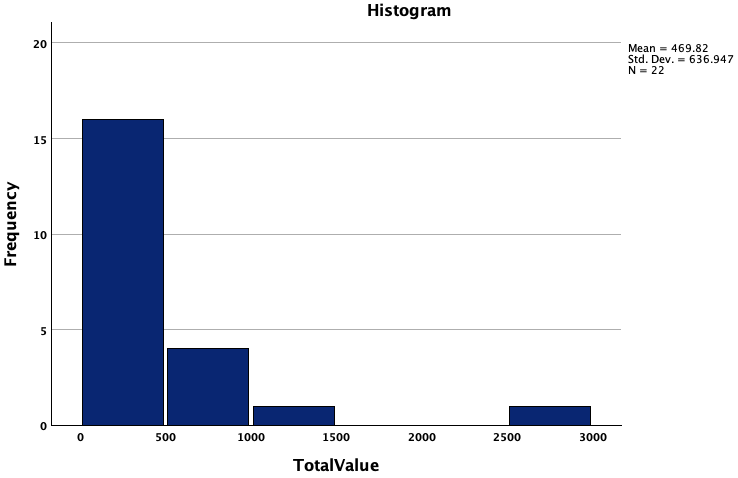
\includegraphics[width=0.8\textwidth]{LAB01/pics/SPSS_Hist.png}%
    \caption{Vẽ Histogram của cột \texttt{Total Value} từ SPSS}
    \label{fig:SPSS_Hist}
\end{figure}

\newpage
\subsection{Sử dụng R}
Từ đoạn code R đã nộp trong file đính kèm, các kết quả được hiện như sau:



\subsection*{Bước 1: Đọc dữ liệu từ file \texttt{VNZ\_STOCK\_DATA\_AUGUST.csv}}

\begin{itemize}
    \item Đặt file \texttt{VNZ\_STOCK\_DATA\_AUGUST.csv} trong cùng thư mục với script R.
    \item Trong R hoặc RStudio, dùng lệnh:
\begin{verbatim}
data <- read.csv("VNZ_STOCK_DATA_AUGUST.csv")
str(data)
summary(data)
\end{verbatim}
    \item Xác định tên cột \texttt{Total Value} trong R là \texttt{Total.Value}, sau đó gán:
\begin{verbatim}
tv <- data$Total.Value
\end{verbatim}
\end{itemize}

\subsection*{Bước 2: Tính các chỉ số Central Tendency}

\begin{itemize}
    \item Mean:
\begin{verbatim}
mean_tv <- mean(tv, na.rm = TRUE)
\end{verbatim}
    \item Median:
\begin{verbatim}
median_tv <- median(tv, na.rm = TRUE)
\end{verbatim}
    \item Mode (tự viết hàm):
\begin{verbatim}
get_mode <- function(x) {
  ux <- unique(x)
  ux[which.max(tabulate(match(x, ux)))]
}
mode_tv <- get_mode(tv)
\end{verbatim}
    \item Quartiles (Q1, Q2, Q3):
\begin{verbatim}
quartiles_tv <- quantile(tv, probs = c(0.25, 0.5, 0.75), na.rm = TRUE)
Q1_tv <- quartiles_tv[1]
Q2_tv <- quartiles_tv[2]
Q3_tv <- quartiles_tv[3]
\end{verbatim}
\end{itemize}

\subsection*{Bước 3: Tính các chỉ số Dispersion}

\begin{itemize}
    \item Variance (sample):
\begin{verbatim}
var_tv <- var(tv, na.rm = TRUE)
\end{verbatim}
    \item Standard deviation:
\begin{verbatim}
sd_tv <- sd(tv, na.rm = TRUE)
\end{verbatim}
    \item Min, Max và Range:
\begin{verbatim}
min_tv <- min(tv, na.rm = TRUE)
max_tv <- max(tv, na.rm = TRUE)
range_tv <- max_tv - min_tv
\end{verbatim}
    \item Standard Error of Mean:
\begin{verbatim}
n_tv <- sum(!is.na(tv))
se_mean_tv <- sd_tv / sqrt(n_tv)
\end{verbatim}
\end{itemize}

\subsection*{Bước 4: Skewness và Kurtosis}

\begin{itemize}
    \item Cài và gọi gói \texttt{e1071}:
\begin{verbatim}
install.packages("e1071")   # chạy một lần
library(e1071)
\end{verbatim}
    \item Tính skewness và kurtosis:
\begin{verbatim}
skew_tv <- skewness(tv, na.rm = TRUE)
kurt_tv <- kurtosis(tv, na.rm = TRUE)
\end{verbatim}
\end{itemize}

\subsection*{Bước 5: In kết quả thống kê ra màn hình}

\begin{verbatim}
cat("===== DESCRIPTIVE STATISTICS FOR TOTAL VALUE =====\n")
cat("Number of observations (n):", n_tv, "\n")
cat("Mean:", mean_tv, "\n")
cat("Median:", median_tv, "\n")
cat("Mode:", mode_tv, "\n")
cat("Q1:", Q1_tv, "\n")
cat("Q2:", Q2_tv, "\n")
cat("Q3:", Q3_tv, "\n")
cat("Variance:", var_tv, "\n")
cat("Standard Deviation:", sd_tv, "\n")
cat("Min:", min_tv, "\n")
cat("Max:", max_tv, "\n")
cat("Range:", range_tv, "\n")
cat("Standard Error of Mean:", se_mean_tv, "\n")
cat("Skewness:", skew_tv, "\n")
cat("Kurtosis (excess):", kurt_tv, "\n")
\end{verbatim}

\subsection*{Bước 6: Vẽ Histogram}

\begin{itemize}
    \item Dùng hàm \texttt{hist}:
\begin{verbatim}
hist(tv,
     main = "Histogram of Total Value",
     xlab = "Total Value",
     col  = "lightblue",
     border = "white")
\end{verbatim}
    \item Có thể chỉnh lại số bins bằng tham số \texttt{breaks}, ví dụ:
\begin{verbatim}
hist(tv,
     breaks = 10,
     main = "Histogram of Total Value",
     xlab = "Total Value",
     col  = "lightblue",
     border = "white")
\end{verbatim}
\end{itemize}

\subsection*{Bước 7: Vẽ Box Plot}

\begin{itemize}
    \item Dùng hàm \texttt{boxplot}:
\begin{verbatim}
boxplot(tv,
        main = "Boxplot of Total Value",
        ylab = "Total Value",
        col  = "orange")
\end{verbatim}
\end{itemize}

\subsection*{Kết quả thu được}

\begin{figure}[!htp]
    \centering
    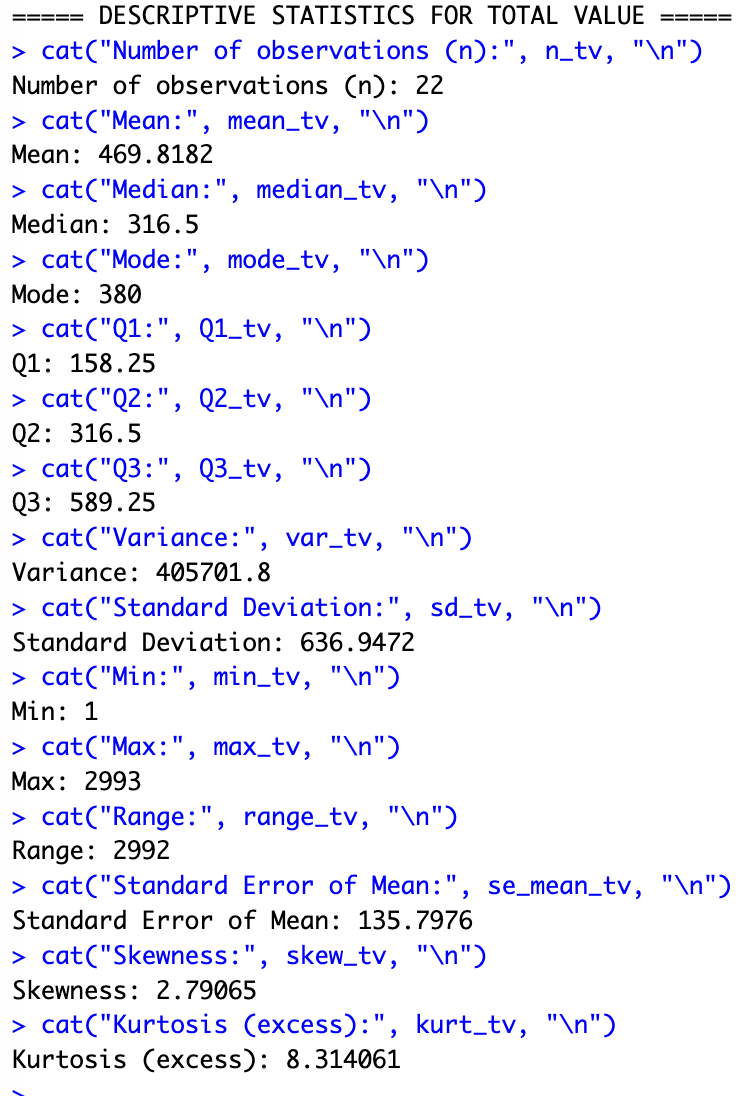
\includegraphics[width=0.57\textwidth]{LAB01/pics/R_Table.png}%
    \caption{Kết quả tính Descriptive Statistics từ R}
    \label{fig:R_Stats}
\end{figure}


\begin{figure}[!htp]
    \centering
    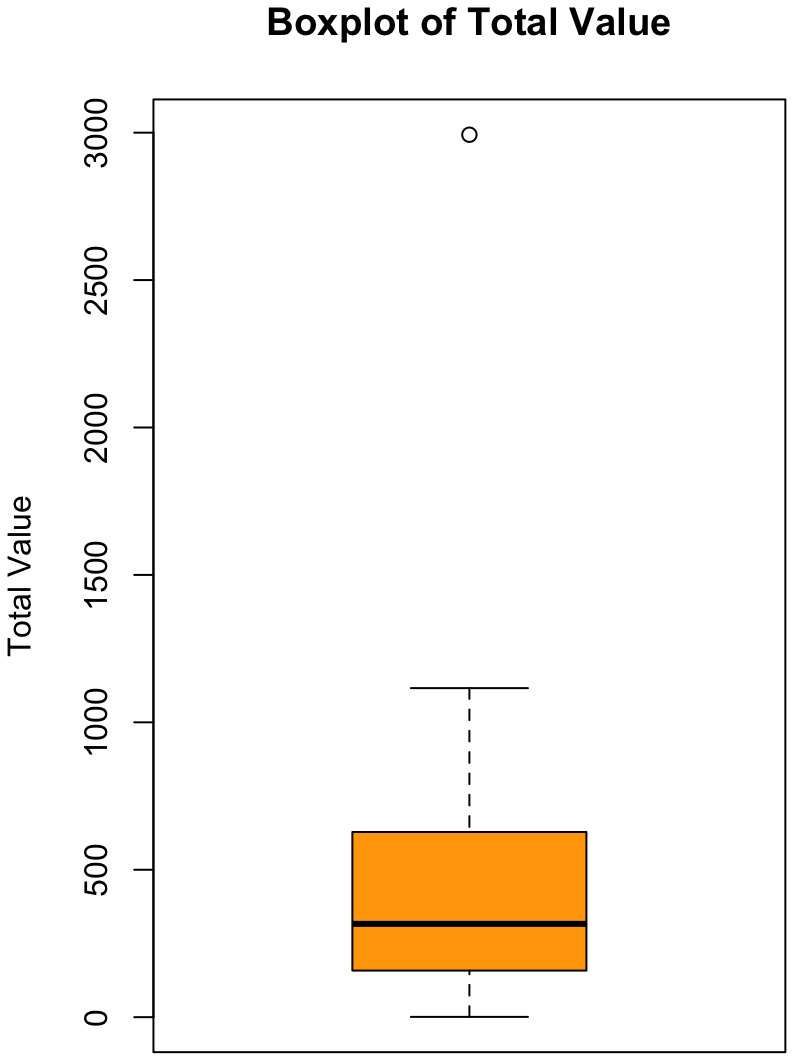
\includegraphics[width=0.4\textwidth]{LAB01/pics/R_BoxPlot.png}%
    \caption{Vẽ BoxPlot của cột \texttt{Total Value} từ R}
    \label{fig:R_BoxPlot}
\end{figure}

\begin{figure}[!htp]
    \centering
    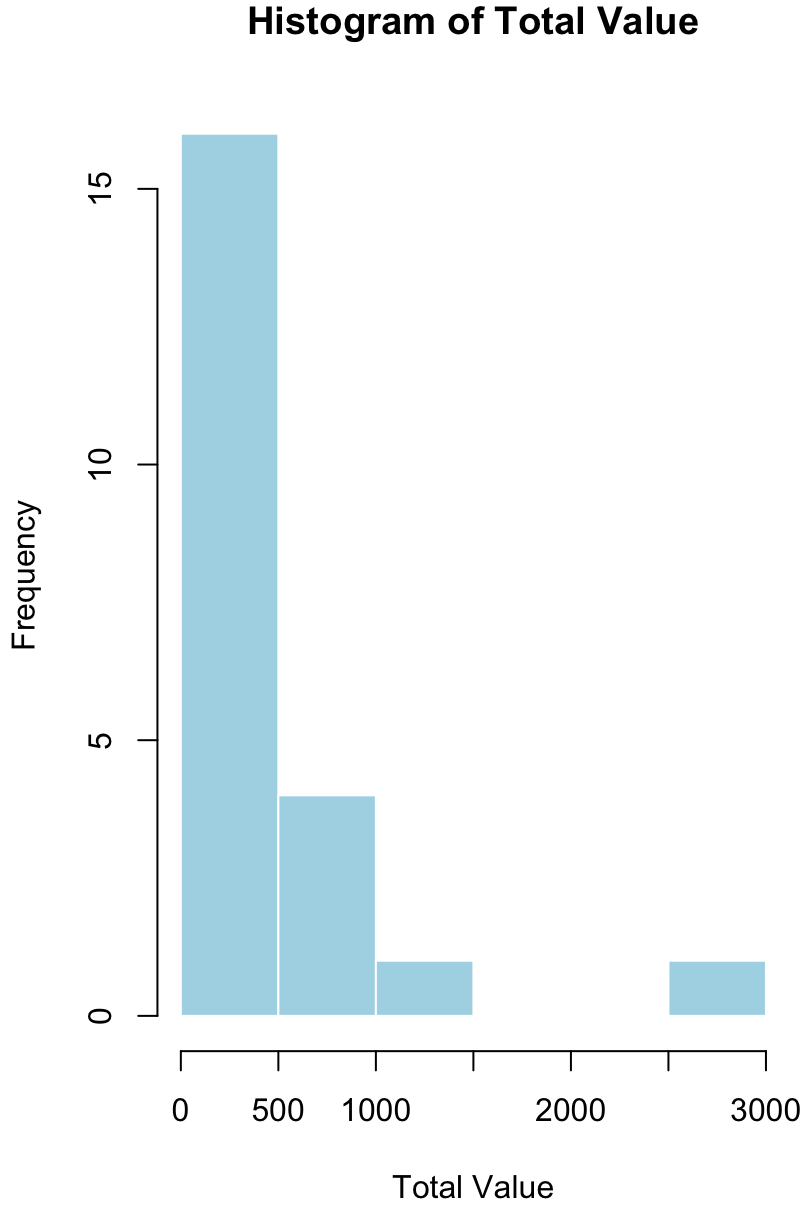
\includegraphics[width=0.5\textwidth]{LAB01/pics/R_Hist.png}%
    \caption{Vẽ Histogram của cột \texttt{Total Value} từ R}
    \label{fig:R_Hist}
\end{figure}


\newpage
\subsection{Sử dụng Python/Jupyter Notebook}

Thực hiện các bước:
\begin{enumerate}
    \item Khai báo thư viện
    \item Import dữ liệu
    \item In ra Descriptive Statistics
    \item Vẽ BoxPlot và Histogram
\end{enumerate}

Sau khi chạy file \texttt{23521449\_Nguyễn Đắc Thành\_LAB01\_Python.ipynb}, thu được các kết quả sau:
\begin{figure}[!htp]
    \centering
    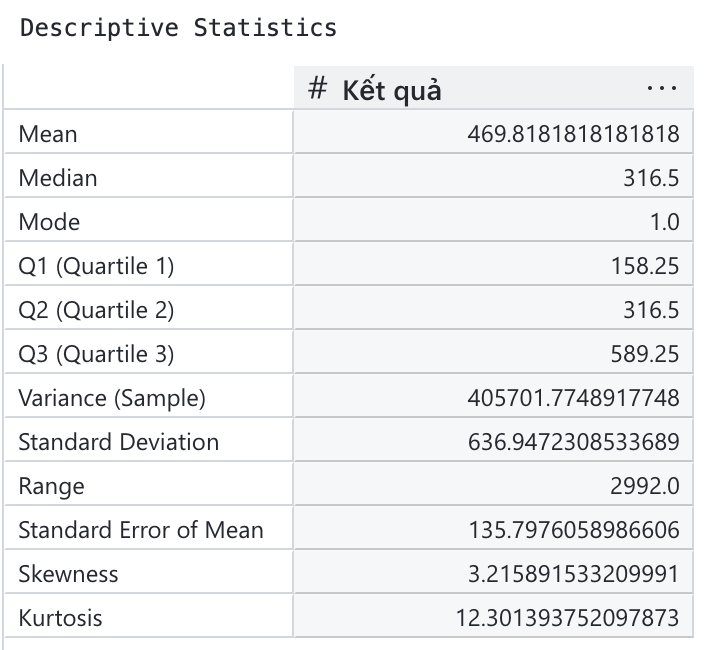
\includegraphics[width=0.5\textwidth]{LAB01/pics/Py_Table.png}%
    \caption{Kết quả tính Descriptive Statistics từ Python}
    \label{fig:Py_Stats}
\end{figure}




\begin{figure}[!htp]
    \centering
    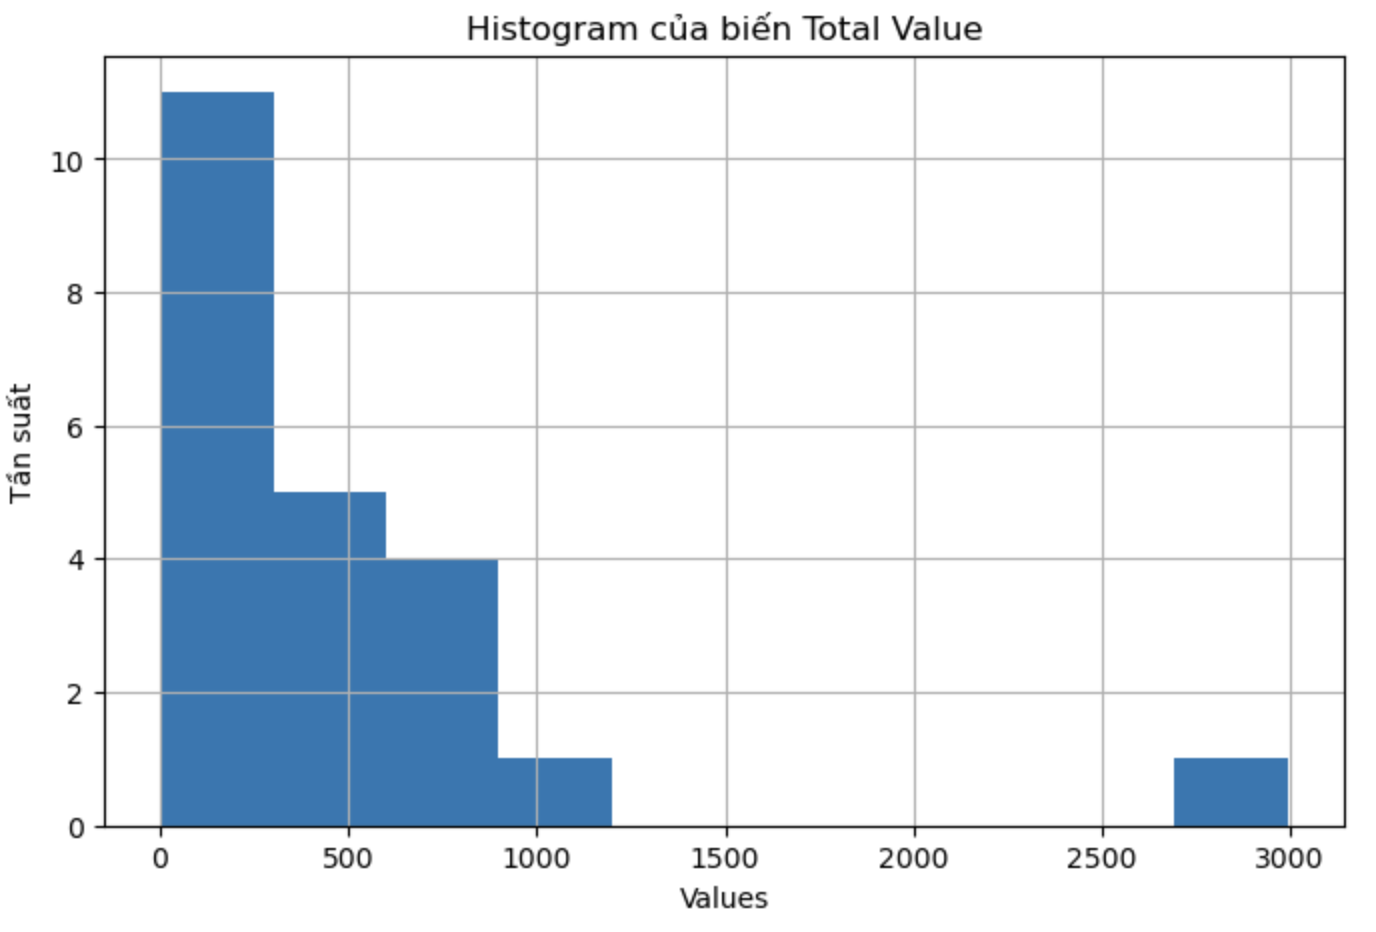
\includegraphics[width=0.56\textwidth]{LAB01/pics/Py_Hist.png}%
    \caption{Vẽ Histogram của cột \texttt{Total Value} từ R}
    \label{fig:R_Hist}
\end{figure}

\begin{figure}[!htp]
    \centering
    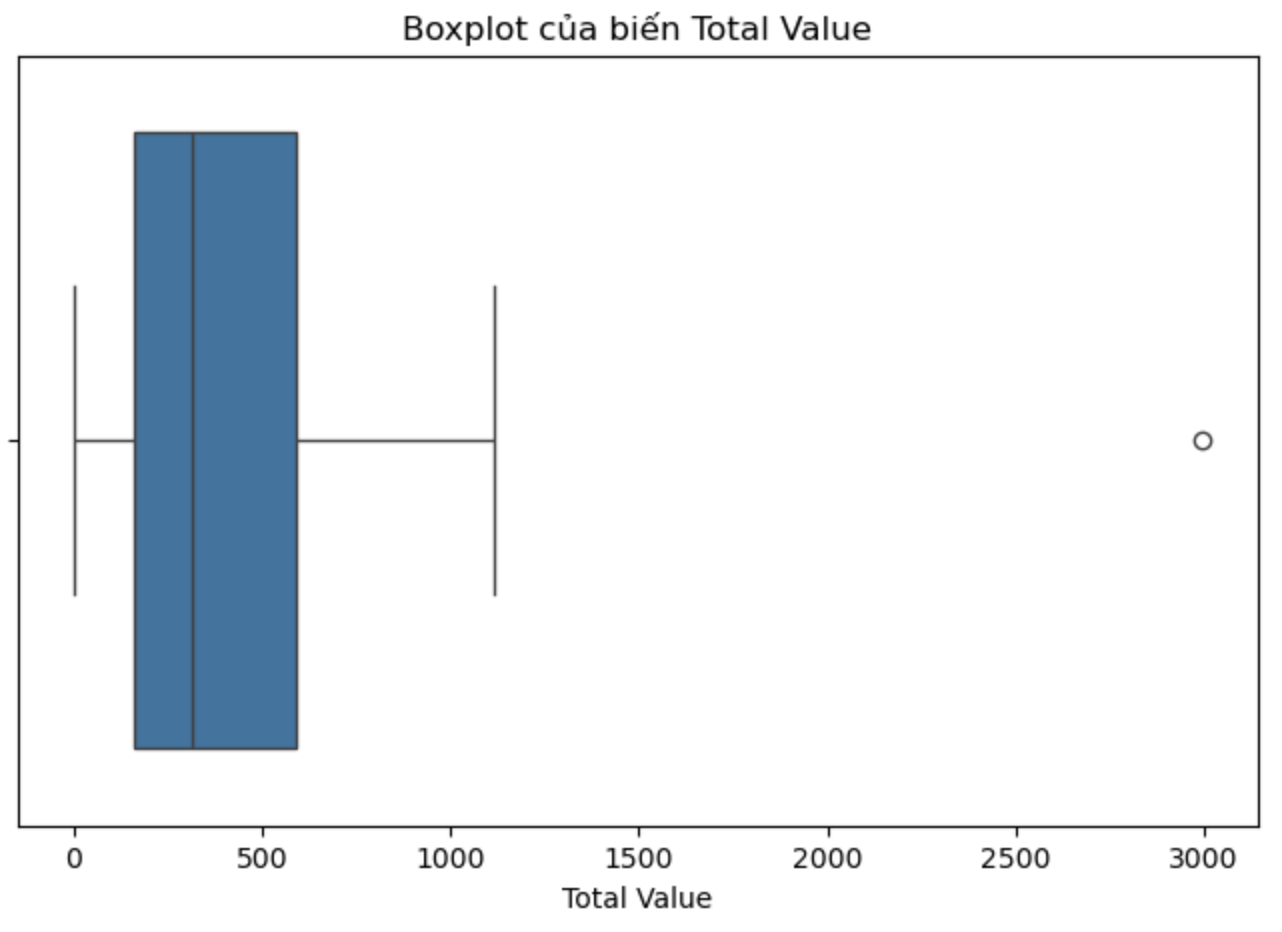
\includegraphics[width=0.6\textwidth]{LAB01/pics/Py_BoxPlot.png}%
    \caption{Vẽ BoxPlot của cột \texttt{Total Value} từ Python}
    \label{fig:Py_BoxPlot}
\end{figure}